\section{eo\-Double\-Exchange Class Reference}
\label{classeo_double_exchange}\index{eoDoubleExchange@{eoDoubleExchange}}
Discrete crossover == exchange of values.  


{\tt \#include $<$eo\-Real\-Atom\-Xover.h$>$}

Inheritance diagram for eo\-Double\-Exchange::\begin{figure}[H]
\begin{center}
\leavevmode
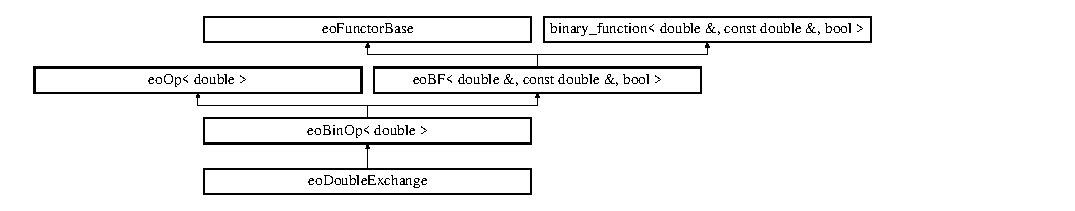
\includegraphics[height=2.38552cm]{classeo_double_exchange}
\end{center}
\end{figure}
\subsection*{Public Member Functions}
\begin{CompactItemize}
\item 
{\bf eo\-Double\-Exchange} ()\label{classeo_double_exchange_a0}

\begin{CompactList}\small\item\em (Default) Constructor. \item\end{CompactList}\item 
virtual std::string {\bf class\-Name} () const \label{classeo_double_exchange_a1}

\begin{CompactList}\small\item\em The class name. Used to display statistics. \item\end{CompactList}\item 
bool {\bf operator()} (double \&r1, const double \&r2)\label{classeo_double_exchange_a2}

\begin{CompactList}\small\item\em Exchanges or not the values. \item\end{CompactList}\end{CompactItemize}


\subsection{Detailed Description}
Discrete crossover == exchange of values. 



Definition at line 41 of file eo\-Real\-Atom\-Xover.h.

The documentation for this class was generated from the following file:\begin{CompactItemize}
\item 
eo\-Real\-Atom\-Xover.h\end{CompactItemize}
